\chapter{Project context}

\section{Introduction}
%In this chapter, we will begin by describing the host company in which our internship is taking place. We will then  shift our focus to the existing system by presenting the current solution and its criticisms in order to extract our key objectives that will guide our project towards a transformative solution.
In this chapter, we are going to start by describing the host company in which our internship is taking place . We will at that point move our focus to the existing framework by presenting the current solution and its criticisms in order to extract our key objectives that will guide our project towards a transformative solution .
\section{Host company presentation}
%In this section, the host company, presented by its logo in the figure 1.1\cite{w1}, Jade Advisory company is presented based on its available informations.
In this section , the host company, presented by its logo within the \textbf{Figure \ref{fig0} } \cite{w1}, Jade Advisory company is presented based on its accessible informations.
\begin{figure}[h]
    \centering
    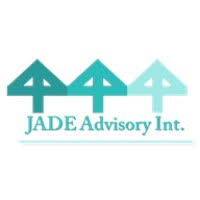
\includegraphics[width=0.3 \linewidth]{assets/jade_advisory.jpg}
    \caption{Jade Advisory logo}
    \label{fig0}
\end{figure}

\subsection{Jade Advisory presentation}
Jade Advisory could be a consulting firm, wich was established since 2019 in Tunis and has included an office in London in 2020, specialized in advising Private and Public entities on structuring , offering and managing framework and PPP projects in Africa and the MENA region.It provides technical advice for the improvement of cost effective, sustainable and innovative solutions competently directing its clients in understanding all technical limitations of the ventures all through their whole life cycle. Its primary concern has continuously been to convey a fulfilling yield to its clients in each project.
%Jade Advisory is a consulting firm, was founded since 2019 in Tunis and has added an office in London in 2020, specialized in advising Private and Public entities on structuring, bidding and managing infrastructure and PPP projects in Africa and the MENA region.It provides technical advice for the development of cost-effective, sustainable and innovative solutions competently guiding its clients in understanding all technical constraints of the projects throughout their entire life cycle. Its main concern has always been to deliver a satisfying output to its clients in each project.
\vskip 0.5cm
\textbf{Figure \ref{fig1} }  illustrate the Distribution of Jade Advisory project over the Africa and the MENA regions.
\begin{figure}[h]
    \centering
    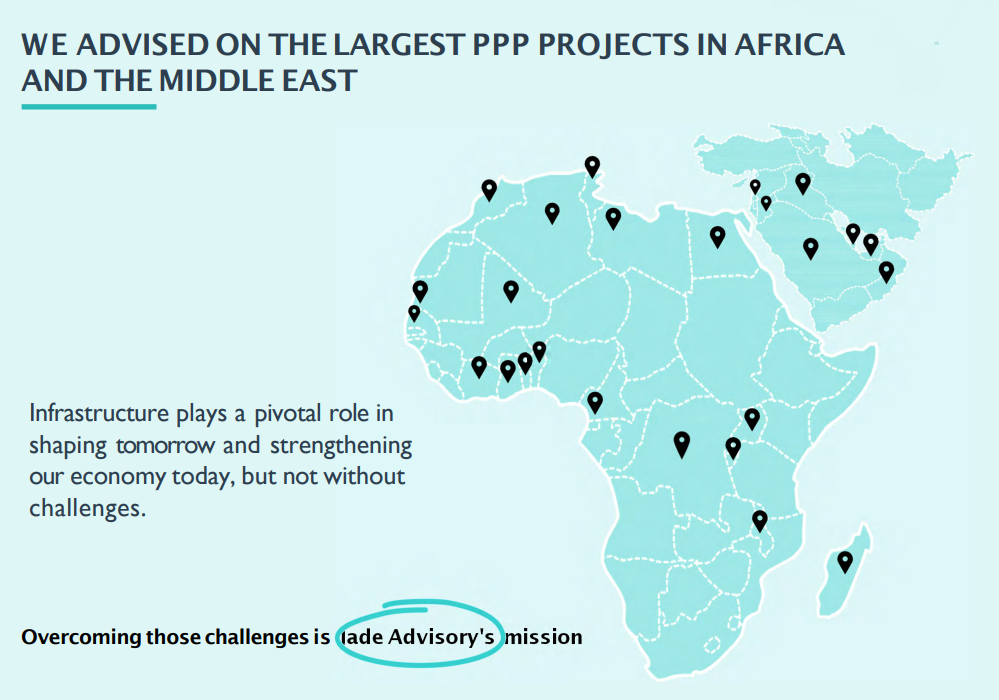
\includegraphics[width=0.9 \linewidth]{assets/jade-reg.png}
    \caption{Distribution of jade advisory projects in the MENA}
    \label{fig1}
\end{figure}

\subsection{Jade Advisory core team}
There are 5 people in the team who are experts in setting up projects that involve public and private partnerships in Africa and the Middle East. The different skills of its international team in strategy, consulting, and PPP services help them give advice that helps businesses grow and make more money. The senior team's skills in English, French, and Arabic help them communicate easily and understand different markets.
%Its dedicated team of five professionals has a proven track record in operationalizing PPP projects across Africa and the Middle East. The diverse expertise of its international team in strategy, consultancy and PPP services ensures it provide insights that drive business growth and profitability. its senior team's proficiency in English, French, and Arabic facilitates seamless communication and understanding across various markets.
\begin{enumerate}
    \item \textbf{Name}: Khaled Amri \\
    \textbf{Role}: Managing Director \\
    \textbf{Background}: Creator of Jade Advisory. Khaled has over 21 years of experience working as a PPP specialist in Europe, the Middle East, and Africa. He used to work at Ernst and Young MENA as a Director in the PPP Team, the French Railway Authority on High Speed Rail PPPs, Commerbank, and General Company Investment Bank in Paris. He has a Master's degree in civil engineering and another Master's in Project Finance and Structured Finance from Ecole of Ponts ParisTech.%Founder of Jade Advisory. Khaled is a PPP specialist with an exeperience of over 21 years in Europe, the Middle East and Africa. He previously worked at Ernst and Young MENA as a Director within the PPP Team, the French Railway Authority on High Speed Rail PPPs, Commerbank and General Company Investment Bank in Paris. He holds a Master's degree in civil engineering and a second Master's in Project Finance and Structured Finance from Ecole des Ponts ParisTech.
    \item \textbf{Name}: Mohamed Amine Sdiri\\
    \textbf{Role}: Director \\
    \textbf{Background}: Mohamed Amine has worked as a Civil Engineer for 11 years in different areas such as international development, government projects, public-private partnerships, and transportation systems. He has a postgraduate diploma in management and international relations from Sciences Po Paris and a Master of Engineering from ENIT Tunisia .%Mohamed Amine is a Civil Engineer with over 11 years of diversified experiences in international development, public sector, PPPs and transport infrastructures. He holds a postgraduate diploma in management and international relations from Sciences Po Paris and a Master of Engineering from ENIT (Tunisia).

    \item \textbf{Name}: Farouk Bouhafs \\
    \textbf{Role}: Senior Consultant \\
    \textbf{Background}: Farouk has a master's degree in Management and Strategy from IHEC Carthage in Tunisia. He has more than 5 years of professional experience in development projects, public private partnerships, project finance and infrastructure advisory. Before joining Jade, Farouk worked as project manager for a consulting company that focuses on helping countries grow and develop.%Farouk holds a master degree in Management and Strategy from IHEC Carthage (Tunisia). He has more than 5 years of professional experience in development projects, public-private partnerships, project finance and infrastructure advisory. Before joining Jade, Farouk worked as project manager for a consulting company specializing in international development.

    \item \textbf{Name}: Houyem Rais \\
    \textbf{Role}: Consultant \\
    \textbf{Background}: Houyem has a bachelor's degree in business administration, with a focus on finance and business analysis, from Tunis Business School TBS . She is a Thomas Jefferson scholarship program (TJSP) alumnus. She started working at Jade Advisory in January 2023.%Houyem holds a bachelor's degree in business administration (Major: Finance, Minor: Business Analysis) from Tunis Business School (TBS). She is a Thomas Jefferson scholarship program (TJSP) alumnus. She joined Jade Advisory in January 2023.

    \item \textbf{Name}: Mohamed Chiheb Tlili \\
    \textbf{Role}: Associate Consultant \\
    \textbf{Background}: Chiheb holds a Master's degree in finance from Mediterranean School of Business. He recently started working as an Associate Consultant at Jade Advisory.%Chiheb holds a Master's degree in finance from the Mediterranean School of Business. He recently joined Jade Advisory as an Associate Consultant. 
    
    
\end{enumerate}



\subsection{Sectors of activity}
Jade Advisory mainly focuses on different areas, as shown in the following \textbf{Figure \ref{fig2} } .
\begin{figure}[H]
    \centering
    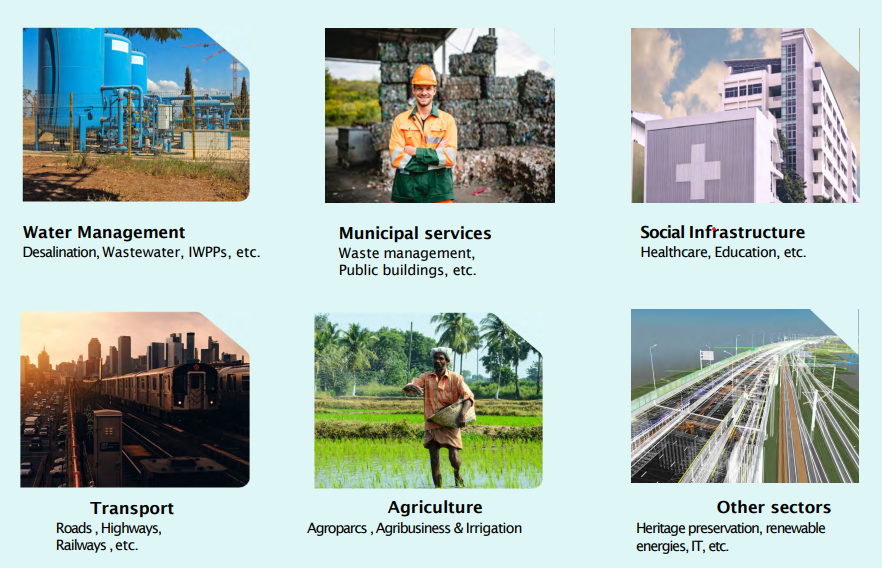
\includegraphics[width=0.9 \linewidth]{assets/jade-sectors.png}
    \caption{Jade Advisory working areas}
    \label{fig2}
\end{figure}
\subsubsection*{Infrastructure Advisory in the transport sector}
%Jade Advisory specialize in delivering comprehensive infrastructure advisory services tailored to the dynamic transport sector. Its expertise serves a diverse clientele, including Private Investors, Governments, International Financial Institutions and Development Agencies. This includes transportation economics, toll management solutions, lifecycle management as well as commercial advisory to physical asset investors, owners, developers and contractors over the project lifecycle, we can see this in table 1.1.
Jade Advisory focuses on providing expert advice on infrastructure for the transport industry. Its
serves many different types of clients, such as Private Investors, Governments, International Financial Institutions, and Development Agencies. This includes transportation economics, toll management solutions, lifecycle management, and commercial advisory for people who invest, own, develop, and build physical assets throughout a project's lifespan, as shown in \textbf{Table \ref{tab0} } .
\begin{table}[H]
    \centering
    \caption{Transport Sector Solutions}
    \label{tab0}
    \begin{tabular}{|>{\raggedright\arraybackslash}p{4.5cm}|>{\raggedright\arraybackslash}p{4.5cm}|>{\raggedright\arraybackslash}p{4.5cm}|}
        \hline
        \rowcolor[gray]{0.8}
        \textbf{Transportation Economics} & \textbf{Toll Management Solutions} & \textbf{Infrastructure Project Lifecycle Management} \\ \hline
        \begin{itemize}
            \item Optimizing financial viability and return on investment (ROI).
            \item Identifying financial risks associated with transportation initiatives and developing tailored mitigation strategies.
            \item Financial modeling and analysis that empowers clients to make well-informed decisions regarding their transportation projects.
        \end{itemize}
        &
        \begin{itemize}
            \item Implementing solutions that maximize revenue collection and financial performance for toll-based transportation projects.
            \item Streamlining toll collection systems and processes, enhancing operational efficiency and reducing costs.
            \item Fostering profitable collaboration between public and private stakeholders.
        \end{itemize}
        &
        \begin{itemize}
            \item Crafting detailed financial roadmaps that guide clients through every stage of infrastructure projects, from inception to completion.
            \item Aligning financing strategies with project milestones, ensuring that financial resources are allocated efficiently.
            \item Developing proactive risk mitigation plans, safeguarding the financial health of infrastructure projects and enhancing investor confidence.
        \end{itemize} \\ \hline
    \end{tabular}
\end{table}




\subsubsection*{Infrastructure Advisory in the water sector}
Jade Advisory uses its knowledge to help with water management. They provide specialized advice on infrastructure to Private Investors, Governments, and Development Agencies. Their main areas of work involve making sure water is used in the best way possible, including finding ways to make seawater usable and managing waste water. We also make sure that our projects are financially sound and that we use water resources efficiently. This can be seen in \textbf{Table \ref{tab1} }.%Jade Advisory leverages its expertise to address the critical water management sector, offering specialized infrastructure advisory services to Private Investors, Governments and Development Agencies. Our focus encompasses water supply optimization, desalination solutions and wastewater management, ensuring financial sustainability and efficient water resource utilization, we can see this in table 1.2.
\begin{table}[h]
    \centering
    \caption{Water Sector Solutions}
    \label{tab1}
    \begin{tabular}{|>{\raggedright\arraybackslash}p{4.5cm}|>{\raggedright\arraybackslash}p{4.5cm}|>{\raggedright\arraybackslash}p{4.5cm}|}
        \hline
        \rowcolor[gray]{0.8}
        \textbf{Water Supply Optimization} & \textbf{Desalination Solutions} & \textbf{Wastewater Management} \\ \hline
        \begin{itemize}
            \item Evaluating water supply projects for economic viability, ensuring sustainable access to clean water for communities
            \item Identifying financial risks in water supply initiatives and developing tailored mitigation strategies
            \item Provide financial modeling and analysis to support innovative water management strategies, optimizing water supply systems for long-term success.
        \end{itemize}
        &
        \begin{itemize}
            \item Implementing cost-effective desalination solutions, providing access to freshwater resources in water-scarce regions.
            \item Streamlining desalination operations, reducing costs and enhancing financial sustainability.
            \item Fostering collaboration between public and private stakeholders to achieve financial success while ensuring reliable desalination services
        \end{itemize}
        &
        \begin{itemize}
            \item Evaluating the financial viability of wastewater management projects, ensuring they meet economic and environmental goals.
            \item Developing financing strategies tailored to the unique needs of wastewater management initiatives.
            \item Promote projects that achieve financial sustainability while advancing responsible wastewater management and environmental protection.
        \end{itemize} \\ \hline
    \end{tabular}
\end{table}

\subsubsection*{Infrastructure Advisory in the waste management sector} 
Jade Advisory helps with waste management. They give advice to different kinds of clients, like private investors, governments, financial institutions, and development agencies. This covers turning waste into resources, following environmental rules, being sustainable, and managing finances during projects. We can find more information in \textbf{Table \ref{tab2} }.
%Jade Advisory extends its expertise to the waste management sector, offering tailored infrastructure advisory services to a wide-ranging client base, encompassing Private Investors, Governments, International Financial Institutions, and Development Agencies. This encompasses waste-to-resource transformation, environmental compliance and sustainability, as well as comprehensive financial project lifecycle management, we can see this in table 1.3.

\begin{table}[H]
    \centering
    \caption{Waste Management Sector Solutions}
    \label{tab2}
    \begin{tabular}{|>{\raggedright\arraybackslash}p{4.5cm}|>{\raggedright\arraybackslash}p{4.5cm}|>{\raggedright\arraybackslash}p{4.5cm}|}
        \hline
        \rowcolor[gray]{0.8}
        \textbf{Waste-to-Resource Transformation} & \textbf{Environmental Compliance and Sustainability} & \textbf{Infrastructure Project Lifecycle Management} \\ \hline
        \begin{itemize}
            \item Optimizing waste management projects for maximum resource recovery.
            \item Identifying opportunities for cost-effective waste-to-resource transformation, enhancing financial performance for both public and private stakeholders
            \item Providing innovative strategies to convert waste into valuable resources, contributing to a circular economy and financial sustainability.
        \end{itemize}
        &
        \begin{itemize}
            \item Optimizing waste management projects for maximum resource recovery.
            \item Identifying opportunities for costeffective waste-to-resource transformation, enhancing financiaperformance for both public and privatstakeholders
            \item Providing innovative strategies to convert waste into valuable resources, contributing to a circular economy  financial sustainability
        \end{itemize}
        &
        \begin{itemize}
            \item Navigating complex environmental regulations and ensuring compliance, mitigating financial risks associated with non-compliance.
            \item Promoting environmentally sustainable waste management practices that reduce long-term financial liabilities and enhance environmental stewardship
            \item Financial modelling and analysis that aligns waste management projects with environmental sustainability
        \end{itemize} \\ \hline
    \end{tabular}
\end{table}

\subsubsection*{Infrastructure Advisory in the social infrastructures sector}
Jade Advisory uses their knowledge to help with important social projects. They offer advice to both private investors and public organizations about infrastructure. This involves making healthcare, schools, and cultural centers better, and improving the community. It helps society grow and be financially stable.
%Jade Advisory brings its expertise to the critical social infrastructure sector, tailoring infrastructure advisory services to Private Investors and Public Entities. This encompasses healthcare infrastructure excellence, educational facilities enhancement, and the development of cultural and community centers, enriching the fabric of society and fostering financial sustainability.



\subsubsection*{Infrastructure Advisory in the agriculture}
%Jade Advisory provides its expertise to the thriving agriculture sector, offering tailored infrastructure advisory services that benefit Private Investors, Farmers, Smallholders, Rural Communities, Governmental Bodies and Development Agencies. This encompasses agroparks development, agribusiness and irrigation, and sustainable rural development, fostering financial sustainability and agricultural excellence.
Jade Advisory helps the growing agriculture industry by giving advice on infrastructure. This helps Private Investors, Farmers, Smallholders, Rural Communities, Government Bodies, and Development Agencies. This includes the growth of agroparks, agribusiness, irrigation, and rural development that helps farmers and communities become financially stable and excel in agriculture.

\section{Project presentation}
In this section, we will talk about current state, what's wrong with it, and suggest ways to make things better and help the business do well.
%In this section, we will outline the current state, critique it, and propose solutions to address challenges and improve enterprise performance.
\subsection{Study of the existing}
Public private partnerships PPPs have become very important in the global infrastructure sector. They help reduce costs and address economic challenges in areas like transportation and energy.
%Public-private partnerships (PPPs) have indeed emerged as indispensable options in the global infrastructure environment, offering promising solutions to lower infrastructure costs and overcome economic constraints in sectors such as transport , energy, and others. 
\vskip 0.5cm
However, using the traditional methods to see if PPP projects are possible can cause some problems. These methods can be tiring, costly, and rely too much on experts, old data, and basic financial models. They provide some useful information but may not be advanced enough to handle the complexity and uncertainty of infrastructure.
%However, traditional methods of feasibility assessment for PPP projects result in distinct inefficiencies. These methods are often laborious, expensive, rely too heavily on expert judgment, historical data, and simple financial models Despite providing some valuable insight, often these methods lack the necessary sophistication required to effectively deal with the complexity and uncertainty of infrastructure.
\vskip 0.5cm
Additionally, as the number of project files and documents increased, organizations like Jade Advisory realized they need for better ways to work together and manage resources. That's why they started using platforms like OneDrive for easier teamwork and improved management. Jade Advisory decided to use ChatGPT as an AI assistant in their work, which can help them better conduct studies and manage project documents. This accreditation involves tasks like reviewing documents, feasibility studies, and asking for advice from experts.
%Additionally, as the volume of project files and documents increased, organizations such as Jade Advisory recognized the need for advanced collaboration and resource management solutions and therefore moved to platforms such as OneDrive in order with easier teamwork and better management. However, Jade Advisory chose to incorporate ChatGPT as an AI assistant in their workflow,which could strengthen their ability to conduct feasibility studies and manage project documentation more efficiently. This accreditation includes activities, including review of documents, feasibility studies, and seeking expert recommendations.
\subsection{criticism of the existing}
% Jade advisory think highly of data privacy, due to sensitive and proprietary information included in its project files .Therefore ,OneDrive isn't a good choice because it is developed and managed by Microsoft. Even if your data is encrypted, Microsoft can get access to it.Otherwise ,communicating documents with chatgpt not only could present  confidentiality issues but also its very slow in term of response speed while dealing with multi-documents on account of the documents curation.
% It's also important to consider the context in which ChatGPT is used and to verify the information it provides through independent sources when necessary, especially in situations where the accuracy and reliability of the information are paramount.
% Jade Advisory lacks a dedicated engineering team or prior expertise. Consequently, ChatGPT might pose a risk by relying on independent sources for information, potentially leading to distractions in its operations, especially in situations where the accuracy and reliability of the information are paramount.

Although public private partnerships PPPs offer promising solutions for building infrastructure, traditional feasibility study methods have many criticisms because they are inefficient and have limitations.
%Although public-private partnerships (PPPs) offer promising solutions in terms of infrastructure development, conventional feasibility study methods face several important criticisms stems from the inefficiencies and various limitations of the current methods.
\vskip 0.5cm
First, using old methods to do feasibility studies with lots of manual work is really hard. These methods are usually slow, require lots of work, and are prone to mistakes. They also cause delays and inefficiencies in decision-making. Relying on expert opinions can lead to subjective and biased results, instead of objective and thorough analysis.
%First, the reliance on traditional methods for conducting feasibility studies, characterized by manual work, presents major challenges. These methods are often time-consuming, labour-intensive and error-prone, in addition to delays and inefficiencies in decision-making processes, their reliance on expert judgment as the primary source of insight encourages subjectivity and bias, and destroys objectivity and robust analysis.
\vskip 0.5cm
Besides, traditional approaches prioritize economic and neglect other important things like social impact, environmental sustainability, and technical development. This limited perspective hinders a full understanding of project feasibility and overlooks potential risks and opportunities that may come from non financial factors.
%Besides, traditional approaches prioritize economic considerations while ignoring other important feasibility considerations, such as social and economic impact, environmental sustainability, and technical development This narrow view limits the broader understanding of project feasibility and ignores potential risks and opportunities that may arise from non-financial factors.
\vskip 0.5cm
Howerver, The absence of automation for everyday tasks like creating reports still causes problems with projects and makes stakeholders less productive.
%However, the lack of automation for common tasks such as report generation continues to contribute to inefficient projects and decrease productivity for stakeholders.
\vskip 0.5cm
Also, ChatGPT's lack of user interaction makes it less efficient and slows down decision-making. Participants may have trouble understanding and using the information given by the AI assistant, which could decrease their effectiveness.
%Furthermore, ChatGPT’s limited user interactivity hinders efficiency and decision making. Participants may have difficulty accessing and interpreting the insights provided by the AI assistant, limiting their ability to fully utilize them.
\vskip 0.5cm
Moreover, the limited access to ChatGPT makes it hard for people with technical skills or disabilities to fully take part in the study. However, the way ChatGPT deals with issues relating to the project, wich is careful and respectful of privacy concerns. Without following strict safety rules, people involved may hesitate to work with AI, which can make the feasibility study process less trustworthy and efficient.
%Furthermore, the limited accessibility of ChatGPT creates barriers for participants with technical skills or disabilities, preventing them from fully participating in the feasibility study process. Nevertheless, how ChatGPT handles related to the project is sensitive to privacy and confidentiality concerns arise. Without strict safety protocols, stakeholders may be reluctant to interact with AI, undermining the integrity and effectiveness of the feasibility study process.
\vskip 0.5cm
In summary, current methods for assessing the feasibility of PPPs have problems like being inefficient, subjective, and only focusing on economic factors. These limits, with difficulties linked to combining data, automating tasks, engaging users, making things easy to access, and protecting privacy. They emphasize the need for a big change in how we make decisions, moving towards more thorough and objective methods.
%In summary, existing feasibility assessment methods in PPPs suffer from inefficiencies, subjectivity, and narrow attention to economic considerations. These constraints, with challenges related to data integration, automation, user interaction, accessibility and privacy. They highlight the necessity for a paradigm shift towards more comprehensive, objective and integrated approaches to ensure robust decision-making.
\vskip 0.5cm
The \textbf{Table \ref{tab5} } shows some possible problems with OneDrive and ChatGPT.
\begin{table}[h!]
    \begin{center}
    \caption{oneDrive and ChatGPT cons}
    \label{tab5}
    \begin{tabular}{{|c|p{0.6\textwidth}|}}
    \hline
     \rowcolor[gray]{0.8}\bfseries Software & \bfseries Cons \\
    \hline
    \raisebox{-1\height}{
\includegraphics[scale = 0.3]{assets/oneDrive.png}} & 
    \begin{itemize}
        \item Weak data privacy.
        \item Data Vulnerability.
        \item Synchronization Limits.
        \item Limited Backup Functionality.
        \end{itemize}\\
     \hline
    \raisebox{-0.9\height}{
\includegraphics[scale = 0.2]{assets/chatgpt.png}} & 
    \begin{itemize}
        \item Provides Inaccurate Information.
        \item Biased Responses.
        \item Limited Knowledge.
        \end{itemize}\\
     \hline
  \end{tabular}
  \end{center}
  
\end{table}


\subsection{Proposed soultion}
To overcome problems with current methods offeasibility assessment in PPPs, we suggest new solutions that use cutting-edge technology to make decisions faster, fairer, and more effective.
%To address the limitations and criticisms of existing approaches to feasibility assessment in PPPs, we propose comprehensive and innovative solutions that use and drive advanced technologies key factors combine to increase efficiency, objectivity and effectiveness in decision-making processes.
\vskip 0.5cm
First of all, Our solution focuses on making it easy for Chat assistance and documents to work together smoothly, allowing data to be exchanged and synchronized seamlessly. This integration will take off the need for people to manually use ChatGPT, make the feasibility study process easier, and boost overall performance. besides, a strong data integration process will be put in place to protect the privacy and confidentiality of important project information.
%First of all, our solution prioritizes seamless integration between Chat assistance and documents, enabling seamless data exchange and synchronization. This integration will eliminate manual interaction with the ChatGPT alternative, simplify the feasibility study process and improve overall performance. Additionally, a robust data integration process will be implemented to ensure the privacy and confidentiality of critical project information.
\vskip 0.5cm
Secondly, we will use technology to make tasks like making reports easier by automating them. Using machine learning algorithms, our solution will help automate comparing reports, saving time and reducing mistakes. This automation will increase productivity so that stakeholders can focus on important tasks that need human skill.
%Secondly, we will add automation capabilities to streamline common tasks such as report generation. Using machine learning algorithms, our solution will automate comparative reporting, reducing manual effort, reducing risk of errors This automation will drive productivity higher to enable stakeholders to focus on higher-value tasks that require human expertise.
\vskip 0.5cm
Thirdly, our solution will have an easy-to-use interface that works well with ChatGPT alternative. We focus on making it easy for people to chat with our assistance, ask questions, and interpreting insights. This better connection will bring together users and make sure that participants can fully utilize the power of AI.
%Thirdly, our solution will provide an intuitive and user-friendly interface, facilitating seamless integration with ChatGPT alternative. We prioritize interactive features that enable participants to effortlessly interact with chat assistance, asking questions, and interpreting insights. This improved connectivity will integrate users and ensure participants can cover the full potential of AI.
\vskip 0.5cm
Our goal is to make sure that our solutions can be used by all people with different skills and abilities. We will give training and support materials to help everyone effectively use the solution.
%Fourthly, we are committed to ensuring that our solutions are accessible to stakeholders with a range of technical skills and abilities. In addition, we will provide comprehensive training and support materials to empower all stakeholders to effectively implement the solution.
\vskip 0.5cm
Our solution will also have strong privacy and confidentiality protections to keep sensitive business data safe. Use encryption, access controls, and audit trails to keep data safe and secure during the analysis process. Make sure to focus on protecting data. Build trust with stakeholders to successfully implement the solution.
%Fifthly, our solution will incorporate robust privacy and confidentiality measures to protect sensitive business data. Implement encryption protocols, access controls and audit trails to ensure data integrity and security throughout the feasibility analysis process Prioritize data security Develop trust and confidence among stakeholders, and to enable the peaceful implementation of the solution.
\vskip 0.5cm
%In summary, our proposed solution provides a holistic approach to address the limitations and criticisms of existing approaches to research in PPPs. By prioritizing data integration, automation, user interactivity, accessibility and privacy, we aim to revolutionize the feasibility analysis process, empowering stakeholders to make decisions.
In summary, our idea offers a complete way to fix the problems with current methods in PPPs.
By focusing on combining data, automation, user engagement, accessibility, and privacy, we want to change how feasibility analysis works and help stakeholders make better choices.
\section{Conclusion}
%We have presented the host company, detailing the core team members and main sectors of activity. Additionally, we have included the presentation of our project, in which we have addressed the existing situation that has been criticized, and then proposed our project solution. Finally, in the next chapter, we will analyze the project's needs.
We have introduced the host company, highlighting the key team members and main areas of work. Moreover, we have included a presentation of our project, in which we have discussed the current issues that have received criticism and then put forward our proposed solution. Finally, in the next chapter, we will look at the project's requirements.